\documentclass{acm_proc_article-sp}

\usepackage{url}
\newcommand{\fixme}{{\bf XXX\ }}

\begin{document}

%don't want date printed
\date{}

%make title bold and 14 pt font (Latex default is non-bold, 16 pt)
\title{Tappan Zee (North) Bridge: Mining Memory Accesses for Introspection}

%\numberofauthors{4}
%
%\author{
%\alignauthor
%Brendan Dolan-Gavitt\\
%    \affaddr{Georgia Institute of Technology}\\
%    \email{brendan@cc.gatech.edu}
%\alignauthor
%Josh Hodosh\\
%    \affaddr{MIT Lincoln Laboratory}\\
%    \email{josh.hodosh@ll.mit.edu}
%\and
%\alignauthor
%Tim Leek\\
%    \affaddr{MIT Lincoln Laboratory}\\
%    \email{tleek@ll.mit.edu}
%\alignauthor
%Wenke Lee\\
%    \affaddr{Georgia Institute of Technology}\\
%    \email{wenke@cc.gatech.edu}
%} % end author

\maketitle

% Use the following at camera-ready time to suppress page numbers.
% Comment it out when you first submit the paper for review.
%\thispagestyle{empty}

\begin{abstract}

The ability to introspect into the behavior of software at runtime is
crucial for many security-related tasks, such as virtual machine-based
intrusion detection and low-artifact malware analysis. Although some
progress has been made in this task by automatically creating programs
that can passively retrieve kernel-level information, two key challenges
remain. First, it is currently difficult to extract useful information
from user-level applications, such as web browsers. Second, discovering
points within the OS and applications to hook for \emph{active
monitoring} is still an entirely manual process. In this paper we
propose a set of techniques to mine the memory accesses made by an
operating system and its applications to locate useful places to deploy
active monitoring, which we call \emph{tap points}. We demonstrate the
efficacy of our techniques by finding tap points for \fixme{number}
useful introspection tasks such as finding SSL keys and monitoring web
browser activity on five different operating systems (Windows 7, Linux,
FreeBSD, Minix and Haiku) and two processor architectures (ARM and x86).

\end{abstract}

\section{Introduction}
\label{sec:introduction}

Many security applications have a need to inspect the internal workings
of software. Host-based intrusion systems, malware analyses, and
digital forensics all depend to some degree on being able to obtain
information about software that is by design undocumented and hidden
from public view. Thus, to operate correctly, security software is
typically built on \emph{reverse engineering}, the art and practice of
elucidating the undocumented principles on which software is built.

Unfortunately, reverse engineering is expensive, time-consuming, and
requires a high degree of expertise. The problem is exacerbated by the
fact that, to protect against tampering, security applications are often
hosted in environments separated from the target being inspected, such
as a separate virtual machine. Because of this, their visibility into
the target is often limited to low-level features such as memory and CPU
state, and any higher-level information must be reconstructed based on
reverse engineered knowledge.

This problem, which we will refer to as the \emph{introspection
problem}, has been approached by a number of recent research efforts
such as Virtuoso~\cite{Dolan-Gavitt:2011uq} and VMST~\cite{Fu:2012fk}.
Existing systems, however, have a number of limitations. First, they
focus on retrieving kernel-level information. However, a great deal of
security-relevant information exists only at user-level, such as URLs
being visited by the browser, instant messages and emails sent by
desktop clients, and system and application log messages. Second,
they require that the desired information be accessible through some
public interface (a public API in the case of Virtuoso, and a userland
program or kernel module in the case of VMST). This means that some
security-relevant information, such as \fixme{example}, may be
inaccessible to such tools. Finally, Payne et al.~\cite{payne:2008}
argue that many security applications need some form of \emph{active
monitoring}; that is, they need to be notified when certain system
events occur. Current solutions to the introspection problem provide no
way of locating places in the system where it would be useful to
interpose.

In this paper, we attempt to address the limitations of past solutions
by examining a rich source of information about system and application
activity: memory accesses observed at runtime. Our key insight is that a
memory access made at a different points in a program \footnote{To deal
with bulk-copy functions such as \texttt{memcpy}, we require a
definition of a program point that is slightly stronger than just the
program counter.  We discuss this in more detail in Section
\ref{sec:technical}.} can be treated as a streams of information that
are likely to be of the same type. For example, when visiting a URL, a
web browser must write to memory the URL that is being visited, and it
will generally do so at the same point in the program; by intercepting
memory accesses made at this program point we can observe all URLs
visited. These program points, which we call \emph{tap points}, provide
a natural place to interpose to extract security-relevant information.

There are a several challenges that must be overcome to make use of tap
points. The first is the sheer amount of data that must be sifted
through. In ten minutes' worth of execution on a Windows 7 system, for
example, we observed a total of 18.9 \emph{million} unique tap points
which read and wrote a total of 32.8 gigabytes of data. To overcome this
challenge, we make use of techniques from information retrieval and
machine learning, described in Section~\ref{sec:technical}, to quickly
zero in on the tap points that read or write information relevant to
introspection.

Second, simply setting up an environment in which one can observe every
memory access made by the whole system (OS and applications) poses a
challenge. Whole-system emulators such as QEMU~\cite{Bellard:2005}
provide the necessary basis for such instrumentation, but intercepting
and analyzing every memory access online is not practical: the resulting
system is so slow that network connections time out and the guest OS may
think that programs have become unresponsive. To solve this problem, we
add \emph{record and replay} to QEMU, which allows executions to be
recorded with low overhead. Our heavyweight analyses are then run on
the replayed execution to analyze every memory access made
\emph{without} perturbing the system under inspection. We describe our
system, Tappan Zee Bridge (TZB),\footnote{Please accept our sincere
apologies for this pun.} in detail in
Section~\ref{sec:implementation}.

Finally, previous systems have required a significant amount of effort
to support new architectures. This problem has become more pressing in
recent years, as ARM-based devices such as smartphones have exploded in
popularity. Because TZB looks at memory accesses, rather than inspecting
binary code, it naturally supports a wide variety of architectures with
minimal effort. To demonstrate this, our evaluation includes the MIPS
and ARM architectures in addition to x86.

The remainder of this paper is structured as follows.
Section~\ref{sec:technical} describes techniques for finding tap points
of interest. We then discuss our system, Tappan Zee Bridge, which
implements these techniques, in Section~\ref{sec:implementation}. We
evaluate TZB in Section~\ref{sec:eval}, and show that it is capable of
finding tap points useful for introspection in a wide variety of
applications, operating systems, and architectures. Finally, we describe
the limitations of our approach in Section~\ref{sec:limitations},
related work in this area in Section~\ref{sec:relwork}, and offer
concluding remarks in Section~\ref{sec:conclusion}.


\section{Applications}

\subsection{Malware Analysis}

As we will show in Section \ref{sec:eval:subsec:supervised}, TZB can be used for malware analysis in some cases.

\subsection{VM-Based Security and Intrusion Detection}

Little bit about comparing network traffic to VM data?

Tap points for SSL interception without man in the middle (more in evaluation section).

\subsection{Debugging}

Maybe mention booting embedded systems here? Find internal log buffers, etc.


\subsection{Modes of Success and Failure}

TZB is a peculiarly simple, but, we believe, elegant solution to the application RE problem.  
At its heart is an assumption.

\emph{For TZB to work, there must exist a set of memory write instructions, which, if monitored, collectively and temporally comprise the contiguous write of the desired data.}

This might appear limiting, a pesky constraint on an otherwise promising technique.
In our experience, it is not; the assumption holds in a surprising number of situations.
We have therefore come to reformulate the assumption as an observation about programs and systems.  

\emph{Application and system introspection buffers containing useful RE information often exist, and when they do, they are likely to be generated by a set of memory writes which collectively and temporally comprise the contiguous write of the desired data.}

We cannot know for certain that the buffers exists, but there are often clues, such as a log file that contains the information, a window that displays it, or a network packet that contains it. 
And, in our experience, when a buffer exists, TZB can usually find the associated tap points and no RE is required.  

Nevertheless, we encountered two contexts in which TZB had difficulty, and they are worth detailing.  
We saw early success in locating the tap points corresponding to Linux kernel messages, and attempted to locate the corresponding tap points on Windows.
These we did not find, using the output of Event Viewer as training examples as described in Section~\ref{sec:technical:subsec:knownunk}.
This is for the simple reason that the desired introspection buffer does not exist.
The kernel writes a log but it uses a compact binary format with message strings indicated by reference ids.
At best, we could hope to use TZB to find a set of tap points corresponding to the buffer containing this binary kernel log.
This is probably feasible. 
But the result would not be human-readable; we would have to employ the Event Viewer to make sense of it.
In this case, we think a more natural approach would be to use OS introspection techniques like Virtuoso~\cite{Dolan-Gavitt:2011uq}.
Given a few training runs of Event Viewer parsing kernel logs and pretty-printing the information, Virtuoso can assemble a python script that performs the same computation from the hypervisor, which access to guest memory and state.
This script can be used to output human readable guest kernel event information whenever desired.

Another challenge to TZB is that calling context depth is difficult to set for all situations.  
Our definition of tap point in Section~\ref{sec:technical:subsec:tapdef} includes the caller address, that is, one level of context.
This is adequate for correctly separating tap point sets that use the same utility function to write data to memory. 
[WAIT -- isn't this solved by the ``contiguous'' requirement?]
However, there are situations in which more or less context can be required, and sometimes no one level is correct.  
We encountered this situation in trying to locate tap points for Linux kernel messages, in which including the caller to the tap point degraded the results slightly.
We considered various schemes but these seemed unprincipled and tricksy.  
Eventually, we decided that fully automating this aspect of the system was unproductive.
Our goal is simply to locate effective tap points quickly.
In many cases, a few minutes of manual examination of results is all that is required to locate the correct tap point sets or identify when a few sets ought to be merged for better results. 
This is quite reasonable compared with alternative of a fully manual technique.


\section{Technical Description}
\label{sec:technical}

To find useful \emph{tap points} in a system---places from which to
extract data for introspection---using Tappan Zee Bridge, one begins by
creating a recording that captures the desired OS or application
behavior. For example, if the end goal is to be notified each time a
user loads a new URL in Firefox, one would create a recording of Firefox
visiting several URLs. This recording is made by emulating the OS and
application inside of TZB, which can capture and record all sources of
non-determinism with low overhead, allowing for later deterministic
replay. Next, one can run one or more analyses that seek out the desired
information among all memory accesses seen during the execution.
Analyses in TZB take the form of plugins that are called on each memory
access made during a replayed execution and, at the end, write out a
report on the tap points analyzed. Finally, the tap points found should
be validated to ensure that they do, in fact, provide the desired
information. Such assurance can be gained either by examining the data
in the tap point in new executions, or by examining the code around the
tap point. This workflow is illustrated in Figure~\ref{fig:workflow}.

In this section, we give a technical description of Tappan Zee Bridge.
We begin by giving a precise definition of a tap point, and discuss the
implications of our choice of definition. Next, we describe three
different ways of finding tap points: searching for ``known knowns'' ---
tap points where the desired data and its format is known; searching for
``known unknowns'' --- tap points where the kind of data sought is known,
but its precise format is not; and finally ``unknown unknowns'' --- tap
points where the type and format of the data sought are not known, and
we are instead simply trying to find ``interesting'' tap points.

\subsection{Defining Tap Points}
\label{sec:technical:subsec:tapdef}

\begin{figure}[t]
\begin{center}
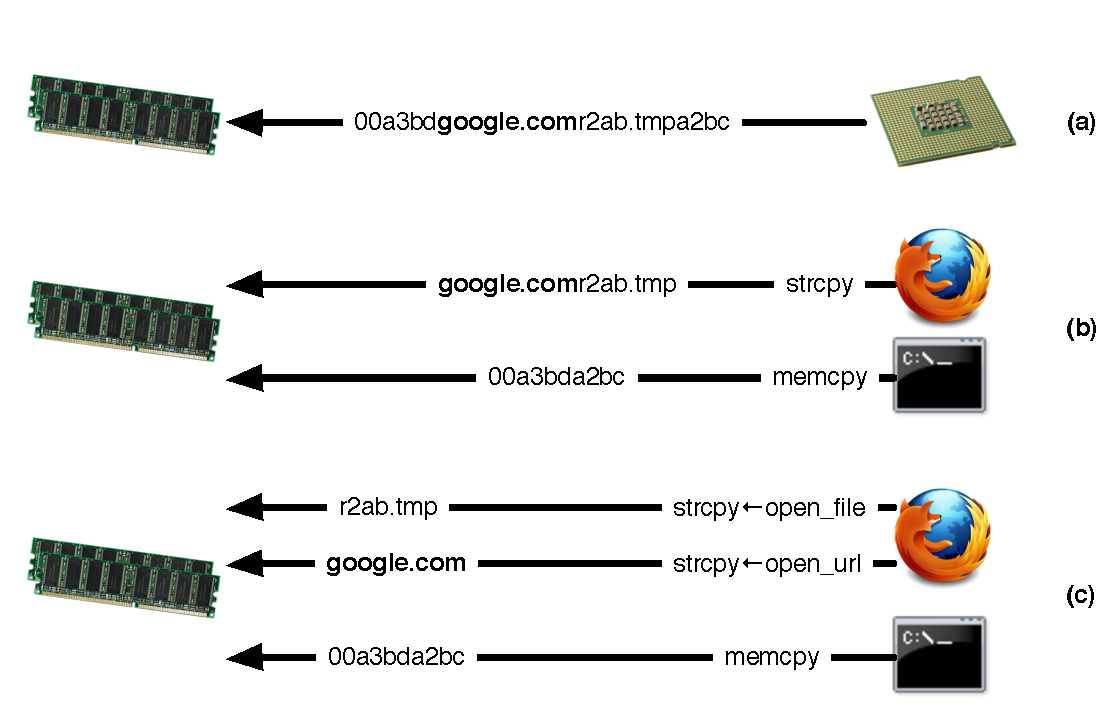
\includegraphics[width=3.2in]{tappoint.pdf}
\end{center}
\caption{Three different ways of defining a tap point: (a) as a single
stream of information from the CPU to RAM ; (b) split up according to
program and location within program ; (c) split up according to program,
location within program, and calling context.}
\label{fig:tappoint}
\end{figure}

A naive approach to defining tap points would be to simply group memory
accesses by the program counter that made them (e.g., EIP/RIP on x86 and
R15 on ARM). However, this approach fails in two common cases: first,
memory accesses made by bulk copy functions, such as \texttt{memcpy} and
\texttt{strcpy}, would all be grouped together, which would commingle
data from different parts of the program into the same tap point. In
addition, looking only at the program counter would conflate accesses
from different programs.

Instead, we define tap points as the triple \[ (caller,
program\_counter, address\_space) \] Including the caller and the
address space (the \texttt{CR3} register on x86, and the \texttt{CP15
c2} register on ARM) separates out memory accesses into streams that
should, in general contain the same type of data. Figure
\ref{fig:tappoint} shows the effect of choosing various definitions of a
tap point when looking for the place where the browser writes the URL
entered by the user (``google.com''). At the coarsest granularity (a),
one can simply look at all writes from the CPU to RAM; however, the
desired information is buried among reams of irrelevant data.
Separating out tap points by program and program counter (b) is better,
but still combines uses of \texttt{strcpy} that contain different
information --- in this case, a filename and a URL. By including the
calling context (c), we can finally obtain a tap point that contains
just the desired information.

Collecting information about the caller is accomplished in TZB in an
architecture-neutral way. Because stack walking is, in general,
unreliable (even on x86, any programs that use frame pointer omission
will cause stack walking to fail), we run a plugin (described in
Section~\ref{sec:implementation:subsec:callstack}) that maintains a
shadow stack based on function calls and returns. This allows us to
generically obtain an accurate call stack at all times, at the cost of
of a slight slowdown in replay performance.

Although it is possible that some tap points may require deeper
information about the calling context (for example, if an application
has its own wrapper around \texttt{memcpy}), we have found that just one
level of calling context is usually sufficient. In addition, because TZB
is a whole-system emulator that can watch every call and return, we can
obtain the call stack to an arbitrary depth for any tap point. This
makes it easy to add extra context for a given tap point, if it is found
that doing so separates out the desired information. An example of a tap
point that requires more than one level of callstack information is
given in Section~\ref{sec:eval:subsec:ssl}.

Conversely, one might wonder whether this definition of a tap point may
split up data that should logically be kept together. To address this
case, we introduce the idea of \emph{correlated tap points}: we can run
a pass over the recorded execution that notices when two tap points
write to adjacent locations in memory. The idea is that these tap points
may be more usefully considered jointly; for example, a single data
structure may have its fields set by successive writes. These writes
would come from different program counters, and hence would be split
into different tap points, but it may be more useful to examine the data
structure as a whole. By noticing this correlation we can analyze the
data from the combined tap point.

\subsection{Known Knowns}

The simplest case is finding data that one knows is likely to be read or
written by a tap point, and where the encoding of the data is easily
guessed. For example, to find a tap point that can be used to notify
the hypervisor whenever a URL is entered in a browser, one can visit a
known sequence of URLs, and then monitor all tap points, searching for
specific byte sequences that make up those URLs. The same holds for
other data whose representation when written to memory is predictable:
filenames, window titles, registry key names, and so on.

To realize this in TZB, we developed a plugin (\texttt{stringsearch})
that can quickly search for byte strings read or written by tap points
during a recorded execution. This can be accomplished with low overhead:
for each string sought and each tap point, we simply keep a counter that
tracks how many characters of the string have been matched so far, and
reset the counter as soon as a non-matching character is found. If this
counter ever equals the length of the string, then we can conclude that
the tap point has read or written the desired information.

\subsection{Known Unknowns}
\label{sec:technical:subsec:knownunk}

A second tap point application involves finding tap points for things
about which we have limited knowledge.

We can easily assemble corpora of exemplars to represent a semantic
class: English prose, kernel messages, or mail headers. These examples
need not come from tap points but can easily be collected directly from
interacting with the operating system itself. From such a corpus, we can
readily build a statistical model of the semantic class. Tap points
whose contents have high likelihood ratios for the semantic model with
respect to a null model are likely to come from the same semantic class
as the corpus. This kind of supervised learning permits us, for
instance, to train a model on examples of the contents of \texttt{dmesg}
under Linux and employ it to locate tap points that write analogous data
in other operating systems such as FreeBSD, Minix, and Haiku.

In TZB, we accomplish this by collecting bigram statistics for all tap
points seen in execution, as well as for the exemplar; the data seen at
each tap point is thus represented as a sparse vector with 65,536
elements (one for each possible pair of bytes). We can then sort the tap
points seen by taking the distance (according to some metric) from the
exemplar. For our metric, we have chosen to use Jensen-Shannon
divergence~\cite{Lin:2006fk}, which is a smoothed and symmetrized
version of the classic Kullback-Leibler
divergence~\cite{Kullback:1951uq} (also known as information gain). We
also examined the Euclidean and cosine distance metrics, but found their
performance to be consistently worse than Jensen-Shannon. Jensen-Shannon
divergence between two probability distributions $P$ and $Q$ is defined
as:

\[
JSD(P, Q) = H \left ( \frac{P+Q}{2} \right ) - \frac{H(P)+H(Q)}{2}
\]

\noindent where $H$ is Shannon entropy.

In addition to statistical comparison to a known exemplar, we can also
search for data of unknown format if we have access to some external
validator. This is the case, for example, when searching for tap points
that write encryption keys: although the exact key may not be known in
advance (ruling out the use of the \texttt{stringsearch} plugin), if we
have bit of encrypted data we can check whether a given byte string is a
valid decryption key.

In TZB, we currently implement this strategy for finding tap points that
write SSL/TLS master secrets, the 48-byte strings from which an
SSL/TLS-encrypted session's keys are derived. In the training phase, we
record the execution of a program that initiates an encrypted connection
to some server; we also record the encrypted packets sent by the client.
Then, using the \texttt{keyfind} plugin, we test each 48 bytes written
by each tap point and see whether the keys derived from it successfully
decrypt a sample packet sent by the client. If so, then we conclude that
the tap point can be used to decrypt SSL/TLS connections made by the
program under inspection. In Section~\ref{sec:eval:subsec:sslmal} we show
how this technique can be used to spy on connections made by the Sykipot
malware, without performing a (potentially detectable) man in the middle
attack.

\subsection{Unknown Unknowns}

The final strategy for finding useful tap points is also the least
focused. If there is no specific introspection quantity sought, one
might instead wish to find interesting tap points, for some suitable
definition of ``interesting.'' To support this scenario, TZB offers a
form of unsupervised learning---clustering---to group together tap
points that handle similar data. The idea is that one can then examine
exemplars from each cluster, rather than being forced to look through a
large number of tap points. Thus, our use of clustering functions as a
form of \emph{data triage}.

Our clustering is based on the venerable $k$-means
algorithm~\cite{Steinhaus:1956kx}, but using the Jensen-Shannon
divergence described in the previous section. As in the statistical
search case, we use bigram statistics for our feature vectors.
Initialization uses the KMeans++ algorithm~\cite{Arthur:2007ve}, which
helps guarantee that the initial cluster centers are widely separated.
We evaluate the performance of this clustering compared to an expert
labeling in Section~\ref{sec:eval:subsec:cluster}.


\section{Implementation}
\label{sec:implementation}

In this section, we describe both the dynamic analysis platform employed to
build TZB, but also TZB-specific algorithmic and data-structure solutions.

\subsection{PANDA}
\label{sec:implementation:subsec:panda}

TZB makes extensive use of the Platform for Architecture-Neutral Dynamic
Analysis (PANDA), which was developed by the authors in collaboration
with (anonymized).

PANDA is based upon version 1.0.1 of the QEMU machine
emulator~\cite{Bellard:2005}. QEMU is an excellent and common choice for
whole-system dynamic analysis for two main reasons. First, performance
is good (about 5x slowdown over native). Second, every basic block of
guest code is disassembled by the host in order to emulate, which means
that there are opportunities to interpose analyses at the basic block or
even instruction level, if desired. QEMU lowers instructions to an
intermediate language (IL) in order to employ a single back-end code
generator, the Tiny Code Generator (TCG). This IL means dynamic analyses
can potentially be written once and re-used for all 14 architectures
supported by QEMU. Further, this version of QEMU is modern enough to be
able to boot and run modern operating systems such as Windows 7 (earlier
versions of QEMU such as 0.9.1 cannot).

There are three main aspects to PANDA that make it very convenient for
building dynamic analyses. First, PANDA provides a plug-in architecture that
readily permits writing guest analyses in C and C++. Plug-in code is
executed from a number of standard callback locations: before and after
basic blocks, memory read and writes, etc. This is not unlike the
schemes employed in other whole-system dynamic analysis platforms such
as BitBlaze~\cite{Song:2008bitblaze} and S2E~\cite{Chipounov:2011s2e}.
In addition, plugins can export functionality that can then be used in
other plugins, allowing complex behavior to be built up from simple
components. From a software engineering perspective, PANDA's plugin
architecture allows the various analyses supported by TZB to be cleanly
separated from the main emulator, which makes for a much more
comprehensible and maintainable codebase.

The second aspect of PANDA that makes it an excellent dynamic analysis
platform is nondeterministic record and replay (RR). In our formulation
of RR, we begin a recording by invoking QEMU's built-in snapshot
capability. Subsequently, we record all inputs to the CPU, including
INs, interrupts, and DMA. Recording imposes a small overhead (10-20\%)
but not enough to perturb execution. During replay, we revert to a
snapshot and proceed to pull CPU inputs from a log when required.
Unlike many other RR schemes, we do not record and replay device inputs,
which means we cannot ``go live'' at any point during replay. But we
can perform repeated replays of an entire operating system under
arbitrary instrumentation load without worrying about this perturbing
application or operating system operation. This capability is vital to
TZB: without record and replay, the heavyweight analyses we perform
would make the system unusably slow.

The final aspect of PANDA worth mentioning is its integration of LLVM.
QEMU lowers basic blocks of guest code to its own IL, which PANDA can,
additionally, re-render as basic blocks of LLVM code via a module 
extracted from S2E. We omit further discussion of this capability
as it is not used by TZB.

\subsection{Callstack Monitoring}
\label{sec:implementation:subsec:callstack}

As explained in Section~\ref{sec:tapdef}, tap points need information
about the calling context. Keeping track of this information requires
some knowledge about the CPU architecture on which the OS is running,
and so we decided to encapsulate this task into a single plugin. TZB's
other analyses can then query the current call stack to arbitrary depth
by invoking \texttt{get\_callers} and not worry about the details
described in this section.

To track call stack information, the \texttt{callstack} plugin examines
each basic block as it is translated, looking for an
(architecture-specific) call instruction (currently, we look for
\texttt{call} on x86 and \texttt{bl} and \texttt{mov lr, pc} on ARM). If
the block includes a call instruction, then we push the return address
onto a shadow stack after each time that block executes.

Detecting the return from a function does not require any
architecture-specific code. Before the execution of every basic block,
we check whether the address we are about to execute is at the top of
the stack; if so, we pop it. We only need to check the starting address
of the basic block, because by definition a return terminates a basic
block, so the return address will always fall at the beginning of a
block.

We note that these techniques may fail if traditional call-return
semantics are violated. For example, if a program emulated calls and
returns by manually pushing the return address and using a direct jump,
it would not be detected as a call. However, for non-malicious
compiler-generated code, we have found that the algorithm described here
works well.

\subsection{Fixed String Searching}
\label{sec:implementation:subsec:stringsearch}

Searching for fixed strings is one of the most effective tools for
finding useful tap points. Because we have to sift through many
gigabytes of data that pass through tap points during any given
execution, it is vital that string search be efficient in both time and
space.

To satisfy these constraints, we developed a string matching algorithm
(implemented as a PANDA plugin called \texttt{stringsearch}) that
requires only one byte of memory per search string and per tap point.
This one-byte counter tracks, for a given tap point, how many bytes of
the search string have been matched by the data seen at the tap point so
far. Whenever a byte is read from or written to memory, we can check
what the next byte in the search string is using this position, and
compare it to the byte passing through the tap point. If it matches, the
counter is incremented; if it does not match, the counter is reset to
zero. When the counter equals the length of the search string, we know
that the search string has passed through the tap point, and we report a
match. Note that because the counter is only one byte, our matcher only
supports strings up to 256 bytes long; this cap could be easily raised
to 65,536 bytes by using a two-byte counter, at the cost of doubling the
memory requirements. Thus far, 256-byte strings have been more than
sufficient.

This effectively implements a very simple deterministic finite automaton
(DFA) matcher. Indeed, we believe that it should be possible to
efficiently implement a streaming basic regular expression matcher that
only an amount of memory logarithmic in the number of states needed to
represent the expression. We leave this generalization to future work,
however.

\subsection{Statistical Search and Clustering}
\label{sec:implementation:subsec:bigram}

Collecting bigram statistics on data that passes through each tap point
is an efficient way to enable ``fuzzy'' search based based on some
training examples, as well as enabling clustering. To implement this
we collect bigram statistics for all tap points seen in execution, as
well as for the exemplar; the data seen at each tap point is thus
represented as a sparse vector with 65,536 elements (one for each
possible pair of bytes).

To search, we can then sort the tap points seen by taking the distance
(according to some metric) from the exemplar. For our metric, we have
chosen to use Jensen-Shannon divergence~\cite{Lin:2006fk}, which is a
smoothed and symmetrized version of the classic Kullback-Leibler
divergence~\cite{Kullback:1951uq} (also known as information gain). We
also examined the Euclidean and cosine distance metrics, but found their
performance to be consistently worse than Jensen-Shannon. Jensen-Shannon
divergence between two probability distributions $P$ and $Q$ is defined
as:

\[
JSD(P, Q) = H \left ( \frac{P+Q}{2} \right ) - \frac{H(P)+H(Q)}{2}
\]

\noindent where $H$ is Shannon entropy.

Bigram collection is done by maintaining, for each tap point, two pieces
of information: (1) the last byte that passed through by the tap point,
so that we can see bigrams that span a single memory access; (2) a
histogram of all byte pairs seen at the tap point. The latter of these
must be maintained sparsely: because our bigrams are based on bytes, a
dense histogram would require 65,536 integers' worth of storage per tap
point. Given that most of the executions examined in this paper contain
upwards of 500,000 tap points, this would require more than 120GB of
memory, which is clearly infeasible (and wasteful, since most of those
entries would be zero).

Instead, we store the histogram sparsely, using a C++ Standard Template
Library \texttt{std::map<uint16\_t,int>}. This keeps memory usage down
without sacrificing any accuracy, but it does introduce some extra
complexity when processing the resulting histograms, as our search
software must support sparse vectors rather than simple arrays. Because
of this additional complexity, we opted to implement the search and
clustering algorithms ourselves, after some initial prototyping using
SciPy's \texttt{sklearn} toolkit.

Our clustering is based on the venerable $k$-means
algorithm~\cite{Steinhaus:1956kx}, but using the Jensen-Shannon
divergence described in the previous section. As in the statistical
search case, we use bigram statistics for our feature vectors.
Initialization uses the KMeans++ algorithm~\cite{Arthur:2007ve}, which
helps guarantee that the initial cluster centers are widely separated.
We evaluate the performance of this clustering compared to an expert
labeling in Section~\ref{sec:eval:subsec:cluster}.

Our statistical search tool is implemented in 246 lines of C++, and
computes the Jensen-Shannon divergence between a training histogram
(dense) and a set of sparse histograms. Our K-Means clustering tool is
481 lines of C++ code, and outputs a clustering of the sparse histograms
using Jensen-Shannon divergence as a distance metric.\footnote{The use
of this distance metric is justified theoretically because
Jensen-Shannon distance is a Bregman divergence~\cite{Banerjee:2005qf}
and empirically because our clustering typically converges after around
30 iterations.} Both tools are multithreaded, which greatly speeds up the
computation.

\subsection{Finding SSL/TLS Keys}
\label{sec:implementation:subsec:keyfind}

We have also implemented a PANDA plugin called \texttt{keyfind}, which
locates tap points that write SSL/TLS master secrets. The SSL/TLS master
secret is a 48-byte string from which an SSL/TLS-encrypted session's
keys are derived; thus, if a tap point that writes the master key can be
found, encrypted network traffic can be decrypted and analyzed.

The plugin operates on a recording in which a program initiates an
encrypted connection to some server and an encrypted packet sent by the
client (captured using, e.g., \texttt{tcpdump}). The \texttt{keyfind}
uses each 48 bytes accessed at each tap point as a trial decryption key
for a sample packet sent by the client. If the decrypted packet's
Message Authentication Code (MAC) verifies that the packet was decrypted
correctly then we can conclude that the tap point can be used to decrypt
SSL/TLS connections made by the program under inspection. In
Section~\ref{sec:eval:subsec:sslmal} we show how this technique can be
used to spy on connections made by the Sykipot malware, without
performing a (potentially detectable) man in the middle attack.


\section{Evaluation}
\label{sec:eval}

In this section, we evaluate the efficacy of our various tap point search
strategies, described in Section~\ref{sec:technical}, in finding tap
points useful for introspection. Our experiments are motivated by
real-world introspection applications, and so for each experiment we
describe a typical application for the tap points found. Each experiment
was also generally performed on a variety of different operating sytems,
applications, and architectures in order to evaluate TZB's ability to
handle a diverse range of introspection targets.

\subsection{File Access}
\label{sec:eval:subsec:file}

\begin{table}
    \centering
    \begin{tabular}{|l|l|l|}
        \hline
        Target & Tap & ASCII? \\
        \hline
        Debian (amd64) & foo & foo \\ 
        Debian (arm) & foo & foo \\
        Windows 7 (x86) & foo & foo \\
        Haiku (x86) & foo & foo \\
        FreeBSD (x86) & foo & foo \\
        \hline
    \end{tabular}
\caption{Tap points found for file access on different operating
systems. The ``ASCII'' column indicates whether the data was written in
ASCII or UTF-16.}
\label{tbl:file}
\end{table}

Monitoring file accesses is a requirement for many host-based security
applications, including on-access anti-virus scanners. Thus, locating a
tap point at which systemwide file accesses can be observed is of
considerable importance. However, because previous approaches to the
introspection problem~\cite{Dolan-Gavitt:2011uq,Fu:2012fk} are limited
to polling the target for information, they cannot be used in this
scenario.

To find such a tap point, we designed a training run that created and
accessed 100 files, each named after ten successive digits of $\pi$. The
introspection targets chosen for this test were: Debian squeeze (amd64),
Debian squeeze (armel), Windows 7 SP1 32-bit, FreeBSD 9.0, and Haiku R1
Alpha 3. We then searched for tap points that wrote strings matching the
ASCII and UTF-16 encodings of the filenames using the
\texttt{stringsearch} analysis plugin. The UTF-16 encodings were
included because it was known that Windows 7 uses UTF-16 for strings
pervasively, allowing us to surmise that filenames would likely be
UTF-16 encoded. Finally, to validate the tap points found, we looked at
all data written by the tap point to ensure that it contained all of the
filenames accessed, and that no other data was mixed in.

The results are shown in Table~\ref{tbl:file}. \fixme{Add commentary
here when the results are in.}

\subsection{URL Access}
\label{sec:eval:subsec:url}

\begin{table}
    \centering
    \small
    \begin{tabular}{|l|l|l|}
        \hline
        Browser & Caller & PC \\
        \hline
        Deb Epiphany (arm) & \texttt{0x411de294} & \texttt{0x41aca974} \\
        Deb Epiphany (amd64) & \texttt{0x7ffff51c73c3} & \texttt{0x7ffff4ec4728} \\ 
        Win7 IE8 (x86) & \texttt{0x6ddc351a} & \texttt{0x6dd92b43} \\
        Win7 Firefox (x86) & \texttt{0x6b551dd8} & \texttt{0x6b1bb561} \\
        Win7 Chrome (x86) &  \texttt{0x74e94a65} & \texttt{0x74e94c3c} \\
        Win7 Opera (x86) &  \texttt{0x6b0ff6c6} & \texttt{0x6af72783} \\
        Haiku WebPositive (x86) & \texttt{0x00253721} & \texttt{0x02859583} \\
        \hline
    \end{tabular}
\caption{Tap points found that write the URL typed into the browser by
the user.}
\label{tbl:url}
\end{table}

As with file access, monitoring visited URLs is likely to be of use to
host-based intrusion detection and prevention systems. For example, an
IDS may wish to verify that outgoing requests were initiated by a human
rather than malware on the users's machine, or match URLs visited
against a blacklist of malicious sites. This poses a challenge for
existing introspection solutions, as URL load notification is not
generally exposed by a public API, and the data resides in a user
application (the browser).

To find URL tap points, we created training executions by visiting a set
of three URLs (Google, Facebook, and Bing) the following operating
systems and browsers: Epiphany on Debian squeeze (armel and amd64);
Firefox 16.0.2, Opera 12.10, and Internet Explorer 8.0.7601.17514 on
Windows 7 SP1 (x86); and WebPositive on Haiku (x86). As with the file
access case, we used the \texttt{stringsearch} plugin to search for the
ASCII and UTF-16 representations of the three URLs, and then validated
each tap point found to ensure that it wrote only the desired data. The
results can be seen in Table~\ref{tbl:url}.

\fixme{We need to fix the caller information for amd64 and arm before
we submit. Also hopefully this will make the Opera result better---right
now each URL gets put into its own tap point, probably because of FPO;
the tap listed does contain every URL, but also contains some extra
infomration.}

\subsection{TLS/SSL Master Secrets}
\label{sec:eval:subsec:ssl}

\begin{table*}
    \centering
    \small
    \begin{tabular}{|l|l|l|l|}
        \hline
        Client & Caller & PC & Process \\
        \hline
        Deb OpenSSL (arm) & unknown & \texttt{tls1\_PRF+0x144} & openssl \\
        Deb OpenSSL (amd64) & unknown & \texttt{tls1\_generate\_master\_secret+0x108} & openssl \\ 
        Deb Epiphany (amd64) & unknown & \texttt{md5\_write+302} & epiphany \\ 
        Win7 Chrome (x86) & \texttt{\_NSC\_DeriveKey+0x1241} & \texttt{\_TLS\_PRF+0xa0} & chrome.exe \\
        Win7 IE8 (x86) & \texttt{\_Tls1ComputeMasterKey@32+0x57} & \texttt{\_PRF@40} & lsass.exe \\
        Win7 Firefox (x86) & unknown & \texttt{\_TLS\_PRF+0xbb} & firefox.exe \\
        Win7 Opera (x86) & \texttt{Opera.dll+0x2eb06e} & \texttt{Opera.dll+0x50251} & opera.exe \\
        \hline
    \end{tabular}
\caption{Tap points found that write the SSL/TLS master secret for each
SSL/TLS connection. These keys can be used to perform transparent
interception of SSL traffic without man-in-the-middle. Note that for
readability we have reported the symbolic names found using debug
symbols (where available); however, this functionality is not a
necessary part of TZB.}
\label{tbl:ssl}
\end{table*}

Monitoring SSL/TLS-encrypted traffic is a classic problem for intrusion
detection systems. Currently, hypervisor- or network- based IDSes that
wish to analyze encrypted traffic must perform a man-in-the-middle
attack on the connection, presenting a false server certificate to the
client. Not only does this require the client to cooperate by trusting
certificates signed by the intrusion detection system, it also takes
control of the certificate verification process out of the hands of the
client---a dangerous step, given that many existing SSL/TLS interception
proxies have a history of certificate trust
vulnerabilities~\cite{JarmocBHEU2012}.

Instead of a man-in-the-middle attack, we can instead use TZB to find a
tap point that reads or writes the SSL/TLS master secret for each
encrypted connection. Because this secret must be generated for each
SSL/TLS connection, if we can find such a tap point, it can then be
provided to the IDS to decrypt and, if necessary, modify the content of
the SSL stream.

To find the location of these tap points, we a modified copy of
OpenSSL's \texttt{s\_server} utility that prints out the SSL/TLS master
key any time a connection is made. We then recorded executions in which
we visited the server with each of our tested SSL clients, and noted the
SSL/TLS master secret. Finally, we used \texttt{stringsearch} to search
for a tap point that wrote the master key, and verified that the tap
wrote exactly one master key per connection. For this test, we used:
OpenSSL s\_client 0.9.8 on Debian squeeze (armel), OpenSSL s\_client
0.9.8 and Epiphany \fixme{version} on Debian squeeze (amd64), and Firefox
16.0.2, Google Chrome 23.0.1271.64, Opera 12.10, and Internet Explorer
8.0.7601.17514 on Windows 7 SP1 (x86). The results are shown in
Table~\ref{tbl:ssl}.

There is one particular point of interest to observe in these results.
In the case of Epiphany on Debian, we found that one level of callstack
information was \emph{not} sufficient, in contrast to the other results
reported here---with only the immediate caller, the tap point contains
more data than just the SSL/TLS master secret. This is because the
version of Epiphany uses SSLv3 to make connections, and the
pseudo-random function (PRF) used in SSLv3 has the form
\[ MD5(SHA1(\ldots))\] The other implementations instead use TLSv1.0,
where the PRF has the form \[ MD5(\ldots) \oplus SHA1(\ldots) \] This final
XOR operation is done from a unique program point, so the tap point that
results from it contains only TLS master keys. This points to a
potential downside of using tap points for introspection: it is not
always clear in advance how many levels of call stack information will
be required.

We were succesful in locating tap points for all SSL/TLS clients tested.
We note that uncovering similar information using traditional techniques
would have required significant expertise and reverse engineering of
both open source and proprietary software.

\subsection{SSL Malware}
\label{sec:eval:subsec:sslmal}

The need to snoop on SSL-encrypted connections arises in malware
analysis as well. Two features distinguish this case from that of
intercepting the traffic of benign SSL clients presented in the previous
section. First, the ability to decrypt the traffic without a man in the
middle is even more important: in contrast to benign clients, we cannot
assume that malware will accept certificates signed by our certificate
authority. Second, we cannot rely on having access to the server's
master secret, as the server is under the attacker's control. This means
that our previous strategy of using a simple string search for the
master secret will not work here.

Instead, we located the tap point in the SSL-enabled malware by creating
a PANDA plugin called \texttt{keyfind} that performs trial decryption on
a packet sent by the malware using each possible 48-byte sequence
written to memory as a key.  Although this is much slower than a string
match, it is the only available option, since the key is not known in
advance.

To test the plugin, we obtained a copy of a version of the Sykipot
trojan released around October 31st, 2012~\cite{sandymal} (MD5:
\texttt{34a1010846c0502f490f17b66fb05a12}). We then created a recording
in which we executed the malware; simultaneously, we captured network
traffic using \texttt{tcpdump}. We noted that the malware made several
encrypted connections to \url{https://www.hi-techsolutions.org/}, and
provided one of the encrypted packets from these connections as input to
the \texttt{keyfind} plugin. The plugin found the same tap point as the
Windows 7 IE8 experiment described in the previous section, indicating
that both the malware and IE8 likely use the same underlying system
mechanism to make SSL connections. The key found was able to decrypt the
connections contained in the packet dump.\footnote{The malware also has
a second layer of encryption, which custom and not based on SSL; we did
not attempt to decrypt this second layer.}

\subsection{Finding \large \texttt{dmesg}}
\label{sec:eval:subsec:dmesg}

\begin{table*}
    \centering
    \small
    \begin{tabular}{|l|l|l|l|l|}
        \hline
        OS & Caller & PC & Kernel? & Rank \\
        \hline
        FreeBSD (x86) & \texttt{msglogstr+0x28} & \texttt{msgbuf\_addstr+0x19a} & Yes & 1 \\
        Haiku (x86) & \texttt{ring\_buffer\_peek+0x59} & \texttt{memcpy\_generic+0x14} & Yes & 1 \\
        Debian (arm) & N/A & \texttt{do\_syslog+0x18c} & Yes & 4 \\
        Debian (amd64) & N/A & \texttt{do\_syslog+0x163} & Yes & 4 \\ 
        Minix (x86) & \texttt{0x190005ee} & \texttt{0x190009d4} & No & 8 \\
        \hline
    \end{tabular}
\caption{Tap points that write the system log (\texttt{dmesg}) on
several UNIX-like operating systems. All tap points were located in the
kernel, except for Minix, which is a microkernel.}
\label{tbl:dmesg}
\end{table*}

System logs are an invaluable resource, both for security and system
administration. In an introspection-based security system, for example,
one might want to find a tap point that contains the system's logs so
that they can be stored securely outside the guest virtual machine.
However, because the format of system logs is particular to each OS, we
need some mechanism that can find tap points that write data that
``looks like'' a log based on an exemplar. The statistical search
described in Section~\ref{sec:technical:subsec:knownunk} is a good fit
for this task: by training on the output of \texttt{dmesg} on one
OS, we can find \texttt{dmesg}-like tap points on other systems.

To locate these system log tap points, we first created a training
exemplar by running the \texttt{dmesg} command on a Debian sid (amd64)
host, and computing the bigram probabilities for the output. We then
created recordings in which we booted five operating systems: Debian
squeeze (armel), Debian squeeze (amd64), Minix R3-2.0 (i386), FreeBSD
9.0-RELEASE (i386), and Haiku R1 Alpha 3 (i386), and computed the same
bigram statistics. We then sorted the tap points seen in each operating
system boot according to their Jensen-Shannon distance from the training
distribution, and manually examined data written by the tap point for
each of the top 30 results in each operating system. Table~\ref{tbl:dmesg}
shows, for each operating system tested, the tap point that we determined to be
the system log, and its rank in the search results.

We can see that in all cases the correct result is in the top 10. There
are two additional features about Table~\ref{tbl:dmesg} that bear
mentioning. First, the reader will note that the two Debian systems have
a caller of ``N/A''. This is because the memory writes that make up
\texttt{dmesg} are done in \texttt{do\_syslog}, which is called from
multiple functions. In these cases, including the caller splits up
information that is semantically the same. We detected this case by
noticing that several of the top-ranked results in the Linux experiments
had the same program counter, and that they appeared to contain
different sections of the same log. Second, the tap point found for
Haiku was also incomplete---some lines were truncated. By using our tap
point correlation plugin, we determined that we were missing a second
tap point that was correlated with the main one; the two together formed
the write portions of a \texttt{memcpy} of the log messages. Once this
second tap point was included, we could see all the log messages
produced by Haiku.

We also attempted to find an analogous log message tap point on Windows
7, but were not successful. This is a result of the way Windows logging
works: rather than logging string-based messages, applications and
system services create a manifest declaring possible log events, and
then refer to them by a generated numeric code. Human-readable messages
are not stored, and instead are generated when the user views the log.
This means that there is no tap point that will contain log messages of
the type used in our \texttt{dmesg} training, and the methods described
in this paper are largely inapplicable unless a training example for the
binary format can be found. However, because there event log query API
is public~\cite{evtquery}, existing tools such as
Virtuoso~\cite{Dolan-Gavitt:2011uq} might be a better fit for this use
case.

Anecdotally, the ability to uncover a tap point that writes the kernel
logs has also been useful for diagnosing problems when adding support
for new platforms to QEMU. For an unrelated research task, we attempted
to boot the Raspberry Pi~\cite{raspberrypi} kernel inside QEMU, but
found that it hung without displaying any output early on in the boot
process. By locating the \texttt{dmesg} tap point, we discovered that
the last log message printed was ``Calibrating delay loop...''; based on
this we determined that the guest was hung waiting for a timer interrupt
that was not yet implemented in QEMU.

\subsection{Clustering}
\label{sec:eval:subsec:cluster}

To test the effectiveness of clustering tap points based on bigram
statistics and Jensen-Shannon distance, we carried out an experiment
that compared the clusters generated algorithmically to a set of labels
generated by two of the co-authors manually examining the data. We
created six recordings representing different workloads on two operating
systems (Windows 7 and FreeBSD 9.0). From FreeBSD, we took recordings of
boot, shutdown, running applications (\texttt{ps}, \texttt{cat},
\texttt{ls}, \texttt{top}, and \texttt{vi}), and a one-minute recording
of the system sitting idle, for a total of four recordings. On Windows
we created two recordings: running applications (\texttt{cmd.exe},
\texttt{dir}, the Task Manager, Notepad), and one minute of the system
sitting idle.\footnote{Although we would have preferred to include
Windows boot and shutdown recordings, at the time our replay system had
a bug (now fixed) that prevented these recordings from being replayed.}
Table~\ref{tbl:clusttaps} shows the number of tap points found in each
of the recordings; we can see that the FreeBSD system is overall much
less active than the Windows 7 system during the time periods we
recorded.

Next, we sampled a subset of the tap points found in each recording.
Given that the vast majority of tap points do not write interesting
information, we opted not to sample uniformly from the all tap points
found. Instead, we performed an initial $k$-means clustering with $k =
100$, and then picked out tap points at various distances from each
cluster center. For each cluster, we chose the tap point at $\sigma$
standard deviations from the center, for $\sigma \in \left\{0, 0.5,
0.75, 1.0, 1.25, 1.5, 1.75, 2.0 \right\}$ for a total of 2,926
samples\footnote{The alert reader will note that this is smaller than
the 4,800 samples one would expect from taking 8 samples from 100
clusters in each of 6 recordings. This is because some clusters did not
have very high variance, and so in many cases there were fewer than 8
samples at the required distance from the center.}. Finally, we dumped
the data from each of the sampled tap points, blinded them by assigning
each a unique id, and then provided the data files to our two labelers.
Each labeler independently assigned labels to each of the samples using
the labels described in Table~\ref{tbl:clustlabels}, and the two
labelers then worked together to reconcile their labels.

Finally, we ran a $k$-means clustering with $k = 10$; $10$ was chosen
because it was a round number reasonably close the number of labels our
human evaluators gave to the data. We then used the Adjusted Rand
Index~\cite{Hubert:1985zr} to score the quality of our clustering
relative to our hand-labeled examples. The Adjusted Rand Index for a
clustering ranges from -1 to 1; clusterings which are independent of the
hand labeling will receive a score that is negative or close to zero. As
can be seen in Table~\ref{tbl:clustqual}, our clustering was generally
of poor quality and did not match up very well on the hand-labeled
samples.

Based on these results, we conclude that at present, clustering does not
appear to work very well for our purposes. There is some hope, however.
In an effort to understand why our clustering performed so poorly, we
created a confusion matrix for the Win7 Apps recording, which can be
seen in Figure~\ref{fig:win7apps}. The values along the diagonal
represent the fraction of taps that were correctly assigned to the
same cluster when a human had assigned them to the same cluster. The
remaining cells represent the fraction of taps correctly assigned to
different clusters when a human had assigned them different labels. The
magenta cells indicate that we did not have enough examples to make a
comparison. In short: light cells mean the clustering performed well on
that pair of labels, dark cells mean it performed poorly. From this we
can see that for many of the labels of human interest (i.e., those which
are primarily text-based) the clustering performed reasonably well,
but it performed poorly on tap points that contained binary data. This
helps explain its poor overall performance, since the vast
majority---90.8\%---of the samples in our labeling were not text-based.
In future work we hope to carry out further experiments to determine
whether the clusters found are

\begin{figure}
    \centering
    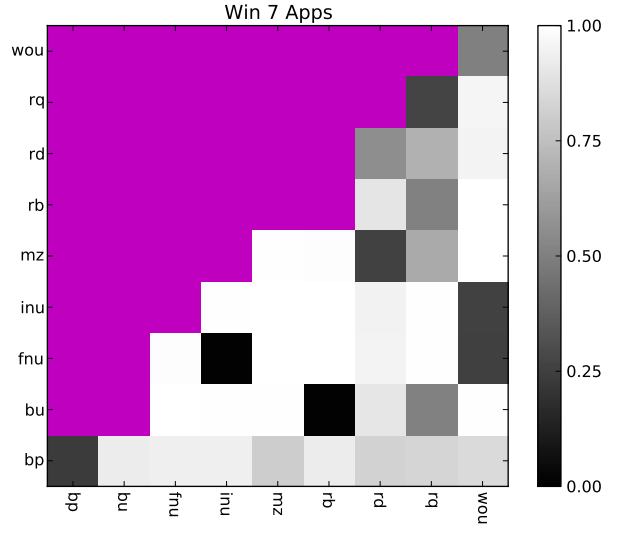
\includegraphics[width=3in]{figures/win7apps.png}
    \caption{Confusion matrix for our clustering of the Windows 7 Apps
    recording compared to handmade labels. Lighter cells indicate that
    the clustering matched the hand-labeled samples well for that
    pair of labels.}
    \label{fig:win7apps}
\end{figure}

\begin{table}
    \centering
    \small
    \begin{tabular}{|l|l|r|}
        \hline
        Abbrv. & Description & Count \\
        \hline
        bp  &  binary pattern &  2318  \\
        rd  &  repeated dword &  400  \\
        mz  &  mostly zero &  141  \\
        rq  &  repeated quadword &  19  \\
        fnu  &  filenames unicode &  8  \\
        woa  &  words ascii &  8  \\
        wou  &  words unicode &  7  \\
        inu  &  integers unicode &  6  \\
        bu  &  binary uniform &  5  \\
        ura  &  URLs ascii &  5  \\
        rs  &  repeated short &  4  \\
        fna  &  filenames ascii &  2  \\
        rb  &  repeated byte &  2  \\
        vr  &  very redundant &  1  \\
        \hline
    \end{tabular}
\caption{Labels given to the sampled tap points by human evaluators,
along with the number of times each occurred.}
\label{tbl:clustlabels}
\end{table}

\begin{table}
    \centering
    \small
    \begin{tabular}{|l|r|}
        \hline
        Recording & Tap Points \\
        \hline
        Win7 Apps        & 1293429 \\
        Win7 Idle        & 520032 \\
        FreeBSD Boot     & 507900 \\
        FreeBSD Shutdown & 152899 \\
        FreeBSD Apps     & 60573 \\
        FreeBSD Idle     & 15569 \\
        \hline
    \end{tabular}
\caption{Number of tap points in each recording.}
\label{tbl:clusttaps}
\end{table}

\begin{table}
    \centering
    \small
    \begin{tabular}{|l|r|}
        \hline
        Recording & ARI \\
        \hline
        FreeBSD Apps & 0.018 \\
        FreeBSD Boot & 0.048 \\
        FreeBSD Idle & 0.021 \\
        FreeBSD Shutdown & 0.074 \\
        Win7 Apps & 0.029 \\
        Win7 Idle & -0.003 \\
        \hline
    \end{tabular}
\caption{Quality of clustering as measured by the Adjusted Rand Index,
which ranges from -1 to 1, with 1 being a clustering that perfectly
matches the hand-labeled examples.}
\label{tbl:clustqual}
\end{table}


\section{Limitations}

Not applicable to memory analysis \\

\noindent
Attacks

\begin{itemize}
\item Split up data reads/writes into noncontiguous chunks and process separately -- obscure semantics
\item Randomize tap locations using something like JIT
\end{itemize}


\section{Related Work}
\label{sec:relwork}

Although, to our knowledge, there is no existing work on mining the
contents of memory accesses for introspection, we drew inspiration from
a variety of sources. These can be roughly grouped into three
categories: work on automating virtual machine introspection, research
on automated reverse engineering, and efforts that examine memory access
patterns, typically through visualization. In this section, we describe
in more detail previous work in these three areas.

Virtual machine introspection has been targeted for automation by
several recent research efforts because of the \emph{semantic gap
problem}: security applications running outside the guest virtual
machine need to reconstruct high-level information from low-level data
sources, but doing so requires knowledge of internal data structures and
algorithms that is costly to acquire and maintain. To address this
problem, researchers have sought ways of bridging this gap
automatically. Virtuoso~\cite{Dolan-Gavitt:2011uq} uses dynamic traces
of in-guest programs to extract out-of-guest tools that compute the same
information. However, because it is based on dynamic analysis,
incomplete training may cause the generated programs to malfunction. Two
related approaches attempt to address this limitation: \emph{process
out-grafting}~\cite{Srinivasan:2011fk} moves monitored processes to the
security VM while redirecting their system calls to the guest VM,
allowing tools in the security VM to directly examine the process, while
VMST~\cite{Fu:2012fk} selectively redirects the memory accesses of tools
like \texttt{ps} and \texttt{netstat} from the security VM so that their
results are obtained from the guest VM. TZB extends these approaches by
finding points in applications and the OS at which to perform active
introspection.

Based on the observation that memory accesses in dynamic execution can
reveal the structure of data in memory, several papers have proposed
methods for automatically deducing the structure of
protocols~\cite{Caballero:2007fk,Lin:2008uq,Cui:2007kx}, file
formats~\cite{Cui:2008ys,Lin:2008vn}, and in-memory data
structures~\cite{Lee:2011,Slowinska:2011ys,Lin:2010}. One particular
insight we have drawn from this body of work is the idea that the point
in a program at which a piece of data is accessed, along with its
calling context, can be used as a proxy for determining the type of the
data. TZB leverages this insight to separate out memory accesses into
streams of data that, are of the same type and often have the same
semantic meaning.

Finally, there has been some research on examining memory accesses made
by a single program or a whole system, typically using visualization.
Burzstein et al.~\cite{Bursztein:2011fk} found that by visualizing
the memory of online strategy games, they could identify the region of
memory used to decide how much of the in-game map was visible to the
player, which greatly reduces the work required to create a ``map hack''
and allow the player to see the entire map at once. Outside the academic
world, the ICU64 visual debugger~\cite{icu64} allows users to visualize
and modify the entire memory of a Commodore 64 system, enabling a
variety of cheats and enhancements to C64 games. Although TZB does not
use visualization, it shares with this previous work the understanding
that memory accesses can be a rich source of information about a running
program.


\section{Conclusion}
\label{sec:conclusion}

In this paper we have presented TZB, a system that automatically locates
candidate memory accesses for active monitoring of applications or operating
systems. This is a task that previously required extensive reverse engineering
by domain experts. We have successfully used TZB to identify a broad range of
tap points, including ones to dynamically extract SSL keys, URLs typed into
browsers, and the names of files being opened. TZB is built atop the QEMU-based
PANDA platform as a set of plug-ins and its operation is operating system and
architecture agnostic, affording it impressive scope for application. This is a
powerful technique that has already transformed how the authors perform RE
tasks. By reframing a diffult RE task as a principled search through streaming
data provided by dynamic analysis, TZB allows manual effort to be refocused on
more critical and less automatable tasks like validation.


\section{Acknowledgments}

A polite author always includes acknowledgments. Thank everyone,
especially those who funded the work. 

\section{Availability}

It's great when this section says that MyWonderfulApp is free software, 
available via anonymous FTP from

\begin{center}
{\tt ftp.site.dom/pub/myname/Wonderful}\\
\end{center}

Also, it's even greater when you can write that information is also 
available on the Wonderful homepage at 

\begin{center}
{\tt http://www.site.dom/\~{}myname/SWIG}
\end{center}

{\footnotesize \bibliographystyle{acm}
\bibliography{biblio}

\end{document}
